    \chapter{Le modèle standard de la physique des particules}

    En physique moderne, l'Univers est gouverné par quatre interactions fondamentales, à savoir l'interaction électromagnétique, l'interaction faible, l'interaction forte et l'interaction gravitationelle. Le modèle standard (MS) est le modèle regroupant les théories quantiques capables de décrire ces interactions \cite{SM1,SM2,SM3}, à l'exception de la gravitation qui à ce jour est décrite par la théorie de la relativité générale d'Albert Einstein et ne possède pas de formulation à l'échelle microscopique. Ainsi le MS fournit une description des \textit{particules élémentaires} et de leurs interactions à travers les outils de la théorie quantique des champs. Après la formulation de la théorie quantique de l'électromagnétisme autour de 1950, les années suivantes ont donné lieu au développement du modèle pour lui donner sa forme actuelle au milieu des années 1970. Depuis, chaque particule prédite au sein du MS a été observée expérimentalement, la dernière découverte étant celle du boson de Higgs en 2012.

    \section{Classification des particules}

    Le modèle standard de la physique des particules comporte deux grandes familles de particules, la première est celle des fermions qui regroupe douze particules de spin $\sfrac{1}{2}$ constitutives de la matière et associées à des champs de Dirac. Elle est elle-même scindée en deux familles avec d'un côté six saveurs de quarks, dont les deux plus légères composent majoritairement les protons et neutrons, et de l'autre six saveurs de leptons dont le plus connu est l'électron. On cite également parmi les fermions l'existence de trois générations contenant chacune deux quarks, dont un de charge électrique $\sfrac{+2}{3}$ et l'autre de charge électrique $\sfrac{-1}{3}$, et deux leptons dont un neutre et un de charge électrique -$1$. La première génération est celle qui forme toute la matière stable avec les quarks up et down, le neutrino électronique et l'électron. Les deux suivantes sont constituées de particules instables se désintégrant rapidement en particules de génération inférieure. À chacune de ces douze particules est également associée une antiparticule constituante de l'antimatière, semblable en tout point à sa jumelle de matière mais avec des nombres quantiques tels que la charge électrique opposés. La symétrie gouvernant l'équité des interactions entre matière et antimatière est appelée symétrie de \textit{Charge-Parité} (CP) et sera discutée dans le chapitre \ref{violCP}.

    \begin{figure}
    \centering
        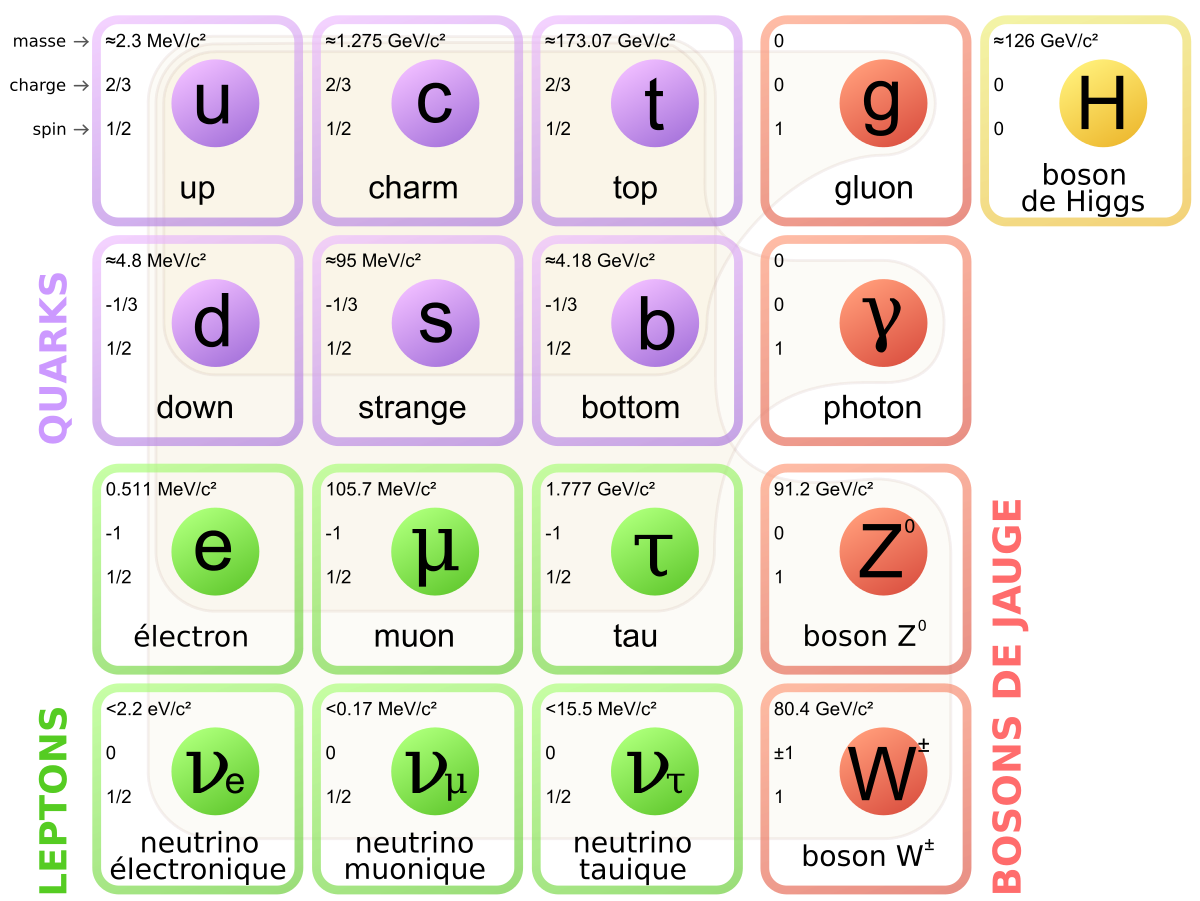
\includegraphics[scale=0.22]{Chapitre2/Images/MS.png} 
        \caption{Représentation graphique du modèle standard. Les douze fermions sont constitués des six quarks (violet) et des six leptons (vert). Chacune des trois générations est formée par une colonne constituée de deux quarks et deux leptons. Les bosons de jauge sont présentés en rouge et le boson de Higgs en jaune.}
    \label{MS}
    \end{figure}

    La seconde grande famille est formée par les bosons de jauge, ou bosons vecteurs, particules de spin $1$ porteuses de force telles qu'introduites dans le paragraphe \ref{sectionQFT} et associées à des champs vectoriels. Parmi celles-ci se trouvent le photon, médiateur de l'interaction électromagnétique, les bosons $W^{\pm}$ et $Z^0$, médiateurs de l'interaction faible et enfin les gluons, médiateurs de l'interaction forte. Finalement, le boson de Higgs est la seule particule du Modèle Standard de spin $0$ et associée à un champ scalaire. Il n'est donc pas une particule médiatrice au sens propre du terme mais entre en jeu dans un mécanisme explicité dans le paragraphe \ref{higgsmeca} à travers lequel les autres particules élémentaires acquièrent une masse. 
    
    \section{Classification des interactions}

    Ce paragraphe est dédié à l'introduction des trois forces fondamentales décrites par le Modèle Standard. Dans un premier temps, une description de la nature de l'interaction sera donnée ainsi que quelques exemples concrets de manifestations physique de ces dernières. Par la suite, chaque Lagrangien sera présenté ainsi que les symétries qui lui sont associées afin de comprendre la nature de chaque interaction à travers quelques diagrammes de Feynman.

        \subsection{Interaction électromagnétique}

        L'interaction électromagnétique est sans doute l'interaction dont les manifestations physiques sont les plus évidentes. Son boson de jauge, le photon, est la particule associée au champ électromagnétique et constitue donc par définition les ondes électromagnétiques quelle que soit leur fréquence, et de cette façon la lumière visible. Dans le cadre de la théorie quantique des champs, l'interaction électromagnétique est capable d'agir sur toute particule élémentaire portant une charge électrique et fait intervenir entre ces dernières l'échange d'un photon sans masse et de charge électrique nulle. \\

        Le Lagrangien de la QED noté $\mathcal{L}_{\tiny QED}$ peut être construit à partir du Lagrangien de Dirac $\mathcal{L}_{\tiny Dirac}$ introduit dans l'équation \ref{Ldirac}. En tentant d'appliquer à un spineur de Dirac libre $\psi$ une transformation du groupe de symétrie U($1$) cette fois locale et non plus globale :

        \begin{equation}
            \psi\rightarrow\psi'=e^{i\chi(\vb{x},t)}\psi,
        \label{localU1}
        \end{equation}

        $\mathcal{L}_{\tiny Dirac}$ se transforme de la façon suivante :

        \begin{equation*}
            \boxed{\overline{\psi}\bigl(i\gamma^{\mu}\partial_{\mu}-m\bigr)\psi}\rightarrow\boxed{\overline{\psi}\bigl(i\gamma^{\mu}(\partial_{\mu}+i\partial_{\mu}\chi)-m\bigr)\psi\ne\mathcal{L}_{\tiny Dirac}}
        \end{equation*}

        et perd ainsi son invariance. Cette dernière peut être conservée en introduisant un \textit{champ de jauge} noté $A_{\mu}$ se transformant selon $A_{\mu}\rightarrow A'_{\mu}=A_{\mu}-\frac{1}{q}\partial_{\mu}\chi$. Le nouveau Lagrangien invariant s'écrit ainsi :

        \begin{equation}
            \mathcal{L}=\overline{\psi}\bigl(i\gamma^{\mu}(\partial_{\mu}+iqA_{\mu})-m\bigr)\psi.
        \end{equation}

        On remarque alors que la conservation de la symétrie du Lagrangien sous une transformation de U($1$) impose l'introduction d'un champ de jauge dont la nature vectorielle implique l'existence d'un boson de jauge de spin $1$ sans masse défini comme le photon. De plus, le théorème de Noether indique la conservation de la grandeur $q$ associée à la charge électrique. D'ores et déjà ce Lagrangien peut être développé afin d'exposer la nature des différents termes qui le composent :

        \begin{equation}
            \boxed{\mathcal{L}=
            i\overline{\psi}\gamma^{\mu}\partial_{\mu}\psi
            -m\overline{\psi}\psi
            -q\overline{\psi}\gamma^{\mu}A_{\mu}\psi}
        \end{equation}

        \begin{enumerate}
            \item[$\bullet$] $i\overline{\psi}\gamma^{\mu}\partial_{\mu}\psi$ : terme cinématique associé aux fermions,
            \item[$\bullet$] $m\overline{\psi}\psi$ : terme de masse associé aux fermions,
            \item[$\bullet$] $q\overline{\psi}\gamma^{\mu}A_{\mu}\psi$ : interaction entre fermions et champ de jauge. \\
        \end{enumerate}

        \begin{figure}
            \centering
            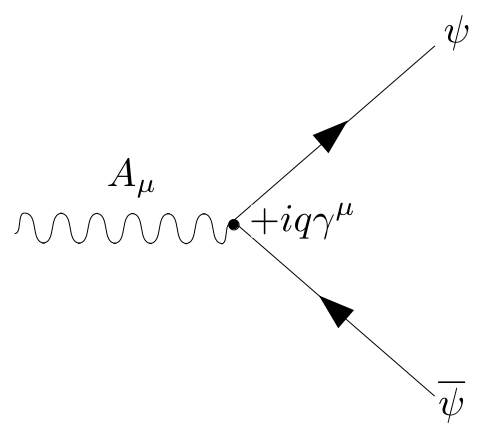
\includegraphics[scale=0.32]{Chapitre2/Images/psiApsi.png} 
            \caption{Vertex issu du terme de couplage du Lagrangien de la théorie électromagnétique quantique.}
        \label{psiApsi}
        \end{figure}

        En particulier, le troisième terme peut être interprété comme un couplage entre un courant de fermion $j^{\mu}=\overline{\psi}\gamma^{\mu}\psi$ tel qu'introduit dans la relation \ref{fermioncurrent} et le champ de jauge $A_{\mu}$. En terme de diagramme de Feynman, ce terme représente un point d'interaction appelé \textit{vertex} entre les champs avec une constante de couplage proportionnelle à la charge électrique $q$ (fig.\ref{psiApsi}). Pour une description complète du nouveau champ de jauge, il faut également ajouter au Lagrangien un terme cinématique et un terme de masse qui lui sont propres au même titre que pour les fermions. Le terme cinématique est directement issu du tenseur électromagnétique $F_{\mu\nu}$ avec pour expression 

        \begin{equation}
            F_{\mu\nu} = \partial_{\mu}A_{\nu}-\partial_{\nu}A_{\mu} 
                       =  \mqty(0 & E_x & E_y & E_z \\ 
                               -E_x & 0 & -B_z & B_y \\
                               -E_y & B_z & 0 & -B_x \\
                               -E_z & -B_y & B_x & 0)
        \end{equation}

        en convention quadrivectorielle $(+,-,-,-)$ et où $E$ et $B$ représentent les champs électrique et magnétique respectivement. \\
        
        Pour être correctement intégré dans le Lagrangien, $F_{\mu\nu}$ doit posséder une forme invariante de Lorentz dont la plus simple s'écrit $-\frac{1}{4}F_{\mu\nu}F^{\mu\nu}$. En revanche, l'ajout d'un terme de masse à la façon des solutions de l'équation de Klein-Gordon de la forme $\frac{1}{2}m^2A_{\mu}A^{\mu}$ brise l'invariance du Lagrangien est impose ainsi une masse nulle pour le photon. Finalement, le Lagrangien pour la QED s'écrit :

        \begin{equation}
            \boxed{\mathcal{L}_{\tiny QED} = \overline{\psi}\bigl(i\slashed{D}-m\bigr)\psi - \frac{1}{4}F_{\mu\nu}F^{\mu\nu},}
        \end{equation}

        avec $\slashed D = \gamma^{\mu}\bigl(\partial_{\mu}+iqA_{\mu}\bigr).$

        \subsection{Interaction faible}
        \label{weakinter}

        L'interaction faible intervient notamment à l'échelle atomique dans des mécanismes de désintégration nucléaire permettant à certains noyaux lourds de retrouver leur stabilité. Historiquement, elle a été introduite en 1930 par Enrico Fermi à travers une interaction à quatre fermions permettant d'expliquer la désintégration $\beta$ du neutron, et plus tard la désintégration du muon en électron observée en 1947. À l'échelle élémentaire, l'interaction faible agit sur les fermions et opère des changements de saveur de ces derniers à travers des courants chargés conduits par les bosons vecteurs $W^{\pm}$. Le couplage entre les bosons $W$ et les fermions possède également la particularité de ne pas conserver la parité. Cette transformation peut être formalisée par un opérateur $\hat{P}$ agissant sur une fonction d'onde en inversant ses coordonnées spatiales : 

        $$\psi(\vb{x},t)\rightarrow\psi'(\vb{x},t)=\hat{P}\psi(\vb{x},t)=\psi(-\vb{x},t).$$

        \begin{figure}
        \centering
            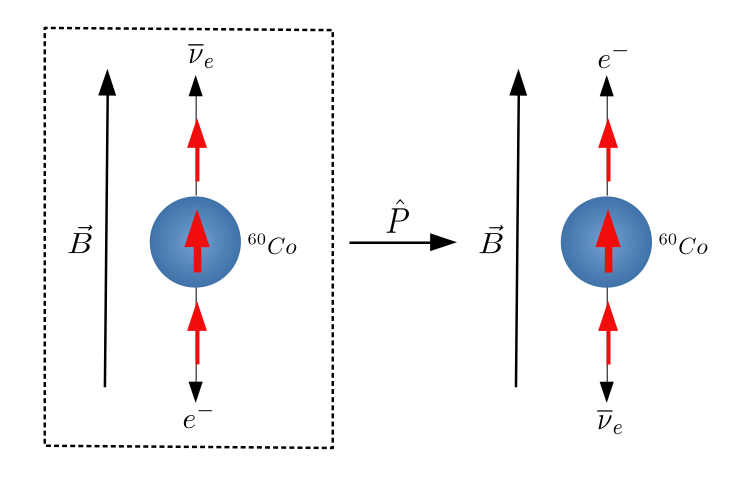
\includegraphics[scale=0.35]{Chapitre2/Images/wuexp.png} 
            \caption{Désintégration $\beta$ du $^{60}Co$. Sous l'action de la parité seules les directions d'émission de l'électron et de l'anti-neutrino sont inversées et la direction du spin est conservée. Seul le processus encadré faisant intervenir un anti-neutrino droit est autorisé.}
        \label{wuexp}
        \end{figure}

        En 1956, Chien-Shung Wu et ses collègues ont mis au point une expérience à travers laquelle des noyaux de cobalt 60 sont placés dans un champ magnétique dans le but d'aligner leurs moments magnétiques à la direction du champ. Dans le référentiel au repos du cobalt, un anti-neutrino et un électron sont émis dans des directions opposées au moment de sa désintégration. Par conservation du spin, chaque fermion possède un spin aligné avec le moment magnétique initial du cobalt. Par transformation de parité, seules les directions des particules émises sont affectées et la direction de leur spin est conservée. La figure \ref{wuexp} illustre les deux scénarios alors possibles. 

        \begin{enumerate}
            \item L'électron est émis dans la direction opposée au champ magnétique avec une impulsion anti-alignée à son spin tandis que l'anti-neutrino est émis dans la direction du champ avec une impulsion alignée à son spin.
            \item L'électron est émis dans la direction du champ magnétique avec une impulsion alignée à son spin tandis que l'anti-neutrino est émis dans la direction opposée au champ avec une impulsion anti-alignée à son spin.
        \end{enumerate}

        Si la parité est conservée, ces deux scénarios se réalisent avec autant de probabilité. Les physiciens ont observé une inhomogénéité dans la direction d'émission des électrons issus de la désintégration $\beta$, avec la direction opposée à celle du champ magnétique fortement favorisée, montrant ainsi que la parité n'est pas conservée par l'interaction faible. \\
        
        L'expérience permet également de montrer qu'à l'inverse l'interaction électromagnétique conserve la parité puisque les photons issus de la désexcitation du noyau de nickel après la désintégration du cobalt sont émis de manière homogène dans l'espace autour du noyau. Ce résultat se reflète dans la structure vectorielle du courant de fermion de l'interaction électromagnétique $j^{\mu}=\overline{\psi}\gamma^{\mu}\psi$, invariant sous la transformation de parité. Le courant faible est quant à lui composé à la fois d'un courant vectoriel et d'un courant pseudo-vectoriel de la forme $\overline{\psi}\gamma^{\mu}\gamma^5\psi$, avec $\gamma^5=i\gamma^0\gamma^1\gamma^2\gamma^3$, dont la combinaison est à l'origine de la violation de parité. L'expérience montre que cette combinaison possède une structure $V-A$ où $V$ est la partie vectorielle et $A$ la partie pseudo-vectorielle donnant lieu à l'expression du couplage faible :

        \begin{equation}
            \boxed{
            \frac{-ig_W}{2\sqrt{2}}\gamma^{\mu}\bigl(1-\gamma^5\bigr),
            }
        \end{equation}

        où $g_W$ est la constante de couplage de l'interaction faible intervenant aux vertex entre fermions et bosons $W^{\pm}$ tels que représentés dans les diagrammes de Feynman de la figure \ref{wdecay}. C'est par ailleurs la petite valeur de cette constante devant celle des autres interactions qui vaut à l'interaction faible son nom.\\
        
        Un autre concept qu'il convient de discuter dans la présentation de l'interaction faible est celui de la chiralité des particules élémentaires. Bien que sans équivalent classique, la chiralité est en réalité la limite ultra relativiste d'une grandeur appelée hélicité représentée par la projection du spin d'une particule sur son impulsion. Une particule dont le spin est aligné à l'impulsion sera dite d'hélicité droite tandis qu'elle sera d'hélicité gauche dans le cas inverse. A travers sa structure, l'interaction faible est capable de se coupler aux particules gauches et aux anti-particules droites uniquement. Mais contrairement à la chiralité, l'hélicité n'étant pas invariante de Lorentz, une particule peut toujours posséder une composante d'hélicité gauche indépendamment de sa chiralité et ainsi se coupler au courant faible, à l'exception du neutrino dont chiralité et hélicité sont toujours confondues en raison de son absence de masse. Il semble toutefois que seul le neutrino gauche et l'anti-neutrino droit soient présents dans la nature, illustrant la non conservation de la parité et la défavorisation du second scénario dans l'expérience de Wu. \\
        
        \begin{figure}
        \centering
            \includegraphics[scale=0.35]{Chapitre2/Images/wdecay.png} 
            \caption{Diagrammes de Feynman associés à la désintégration du muon (gauche) et à la désintégration $\beta^{+}$ (droite).}
        \label{wdecay}
        \end{figure}

        Historiquement, il a également été remarqué que la section efficace de production du processus de diffusion e$^+$e$^-\rightarrow W^+W^-$, reliée à sa probabilité d'occurrence, présente une divergence si seuls les diagrammes impliquant les particules connues à cette époque sont considérées. Cette divergence peut toutefois être corrigée par l'introduction d'un nouveau courant neutre conduit par le boson $Z^0$ tel que présenté dans les diagrammes de la figure \ref{eescat}. Le courant neutre sera finalement observé pour la première fois par l'expérience Gargamelle en 1973, dix ans avant la découverte du boson $Z^0$ en 1983. Son existence fut quant à elle prédite au cours des années 1960 dans le cadre de la théorie électrofaible, unifiant les interactions électromagnétique et faible et offrant un cadre théorique fondé sur la théorie quantique des champs. Une présentation de cette théorie sera donnée dans le paragraphe \ref{EWK} qui lui est consacré.

        \begin{figure}
        \centering
            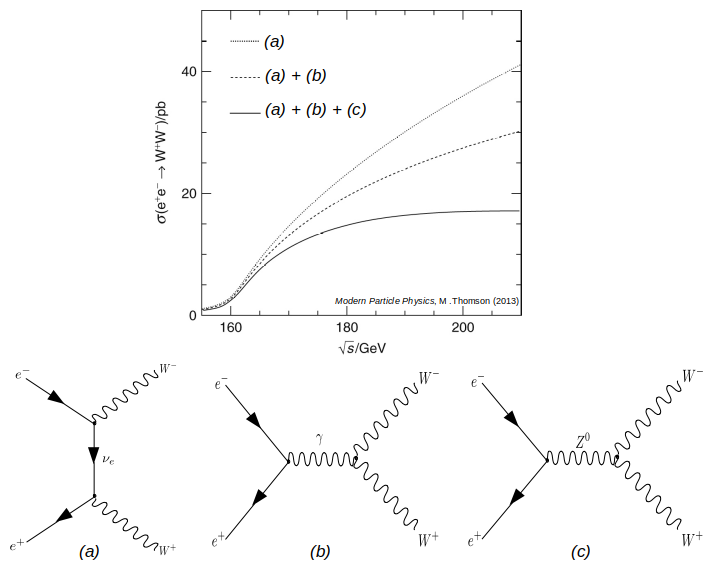
\includegraphics[scale=0.45]{Chapitre2/Images/eescatt.png} 
            \caption{Section efficace de production du processus e$^+$e$^-\rightarrow W^+W^-$ en fonction de l'énergie dans le centre de masse de la paire e$^+$e$^-$. La section efficace diverge si le courant neutre n'est pas considéré.}
        \label{eescat}
        \end{figure}
    
        \subsection{Interaction forte}
        \label{QCD}
        
        L'interaction forte permet notamment de décrire les interactions au sein du noyau atomique et assure la cohésion de celui-ci grâce à une action attractive qui permet de contenir les effets répulsifs des interactions coulombiennes entre protons. Elle permet également la constitution même des nucléons en agissant de la même façon sur les quarks qu'ils contiennent. Il s'agit aussi de la seule force dont l'énergie potentielle d'interaction est assimilable à celle d'un ressort avec une liberté asymptotique et résultant dans le confinement des quarks ne pouvant alors exister à l'état libre. La théorie quantique des champs décrivant l'interaction forte se nomme QCD (\textit{Quantum Chromodynamics}) et décrit son action sur les particules dotées d'une charge dites de \textit{couleur}, dont seuls les quarks sont dotés, à travers l'échange de gluons. \\

        Le Lagrangien de la QCD noté $\mathcal{L}_{\tiny QCD}$ peut être construit sur des principes similaires à ceux utilisés pour construire le Lagrangien de la QED en appliquant cette fois une transformation locale du groupe de symétrie SU($3$) telle que 

        \begin{equation}
            \psi\rightarrow\psi'=\exp[ig_S\vb*{\alpha}(\vb{x},t)\cdot\hat{\vb{T}}]\psi,
        \end{equation}

        où $\hat{\vb{T}}=\{T^a\}$ représente les huit générateurs de SU($3$) construits à partir des huit matrices de Gell-Mann données dans l'encadré \ref{gellmann} selon la relation

        $$T^a=\frac{1}{2}\lambda^a.$$

        \begin{figure}
        \begin{equation*}
        \boxed{
            \begin{array}{cc}
                    \lambda_1=\mqty(0&&1&&0 \\ 1&&0&&0 \\ 0&&0&&0), \quad
                    \lambda_2=\mqty(0&&-i&&0 \\ i&&0&&0 \\ 0&&0&&0), \quad
                    \lambda_3=\mqty(1&&0&&0 \\ 0&&-1&&0 \\ 0&&0&&0), \quad 
                    \vspace{8pt} \\
                    \lambda_4=\mqty(0&&0&&1 \\ 0&&0&&0 \\ 1&&0&&0), \quad
                    \lambda_5=\mqty(0&&0&&-i \\ 0&&0&&0 \\ i&&0&&0), \quad
                    \lambda_6=\mqty(0&&0&&0 \\ 0&&0&&1 \\ 0&&1&&0), \quad 
                    \vspace{8pt} \\
                    \lambda_7=\mqty(0&&0&&0 \\ 0&&0&&-i \\ 0&&i&&0), \quad
                    \lambda_8=\frac{1}{\sqrt{3}}\mqty(1&&0&&0 \\ 0&&1&&0 \\ 0&&0&&-2). \quad
            \end{array}
        }
        \end{equation*}
        \caption{Matrices de Gell-Mann.}
        \label{gellmann}
        \end{figure} 

        La dimension $3\times3$ des matrices de Gell-Mann impose à la fonction d'onde de contenir trois degrés de liberté associés à chacune des charges de couleur : rouge ($r$), verte ($g$) et bleue ($b$). Le maintient de l'invariance du Lagrangien de Dirac requiert alors l'introduction de huit nouveaux champs de jauge $G_{\mu}^{a=1\cdots8}$ associés aux gluons et se transformant selon

    \begin{equation}
        G_{\mu}^{a}\rightarrow G_{\mu}^{a'}=G_{\mu}^{a}-\partial_{\mu}\alpha_a-g_Sf_{abc}\alpha_aG_{\mu}^{b}.
    \label{glutrans}
    \end{equation}

    Le Lagrangien de Dirac devenu invariant sous une transformation locale du groupe SU($3$) s'écrit alors :

    \begin{equation}
        \mathcal{L}=\overline{\psi}\bigl(i\gamma^{\mu}(\partial_{\mu}+ig_SG_{\mu}^aT^a)-m\bigr)\psi.
    \end{equation}

    Ce Lagrangien contient, au même titre que la QED, un terme d'interaction entre les champs associés aux huit gluons et les fermions proportionnel à la constante de couplage de l'interaction forte $g_S$ et dérivé des courants de fermions. En revanche, les termes supplémentaires contenus dans la transformation des champs $G_{\mu}^a$ (éq. \ref{glutrans}) proviennent de la non commutation des matrices de Gell-Mann faisant de la QCD une théorie de jauge non abélienne et donnant naissance à des termes d'auto-interaction des gluons. Les diagrammes de Feynman issus des différents termes d'interaction du Lagrangien sont présentés dans la figure \ref{QCDdiag}. \\

    \begin{figure}
    \centering
        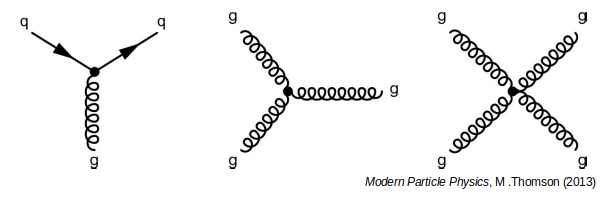
\includegraphics[scale=0.5]{Chapitre2/Images/QCDdiag.png} 
        \caption{Diagrammes de Feynman associés aux termes d'interaction et d'auto-interaction des gluons.}
    \label{QCDdiag}
    \end{figure}

    Finalement, la cinématique associée aux champs des gluons est contenue dans un tenseur de force $F^a_{\mu\nu}$ correspondant à la forme généralisée du tenseur électromagnétique pour une théorie non abélienne :

    \begin{equation}
        F^a_{\mu\nu}=\partial_{\mu}G^a_{\nu}-\partial_{\nu}G^a_{\mu}+g_Sf^{abc}A_{\mu}^bA_{\nu}^c
    \end{equation}

    dont la forme invariante de Lorentz la plus simple s'écrit $-\frac{1}{4}F^a_{\mu\nu}F^{a,\mu\nu}$. Le Lagrangien associé à la QCD prend alors la forme finale :

    \begin{equation}
    \boxed{
        \mathcal{L}_{\tiny QCD}=\overline{\psi}\bigl(i\slashed{D}-m\bigr)\psi - \frac{1}{4}F^a_{\mu\nu}F^{a,\mu\nu},
    }
    \end{equation}

    avec $\slashed D = \gamma^{\mu}\bigl(\partial_{\mu}+ig_SG^a_{\mu}T^a\bigr).$
    
    \section{Brisure de symétrie et unification électrofaible}
    \label{EWK}

    Un des buts fondamentaux des physiciens est de fournir une description unifiée des forces fondamentales de l'Univers. Au cours des années 1960, Sheldon Glashow, Abdus Salam et Steven Weinberg sont parvenus à fournir une description théorique unifiée de l'interaction électromagnétique et de l'interaction faible à travers un modèle dans lequel les deux interactions apparaissent comme deux aspects d'une seule, nommée interaction électrofaible. Au premier abord ces deux interactions semblent toutefois fondamentalement différentes avec d'une part un photon non massif de portée infinie et d'autre part trois bosons massifs de portée comparativement infiniment courte. Un éclairage peut être donné en analysant le groupe de symétrie associé à l'interaction faible. Par analogie à la transformation locale du groupe U($1$) \ref{localU1} introduite pour l'électromagnétisme, l'interaction faible émerge d'une transformation locale du groupe de symétrie SU($2$) :

    \begin{equation}
        \varphi\rightarrow\varphi'=\exp[ig_{W}\vb*{\alpha}(\vb{x},t)\cdot\vb{T}]\varphi,
    \label{localSU2}
    \end{equation}

    où $\vb{T}=\frac{1}{2}\vb*{\sigma}$ représente les trois générateurs du groupe SU($2$) constitués des matrices de Pauli $\sigma$. Cette transformation implique alors cette fois l'existence de trois bosons de jauge associés aux champs $W^{(1)}$, $W^{(2)}$ et $W^{(3)}$ pour satisfaire l'invariance du Lagrangien. De plus, la forme des matrices de Pauli impose à la fonction d'onde $\varphi$ de constituer un doublet dans lequel sont placés les deux fermions entre lesquels les courants chargés opèrent un changement de saveur en attribuant à chacun une charge d'isospin faible $I_W^{(3)}=\pm\sfrac{1}{2}$ pour une charge d'isospin faible totale du doublet $I_W=\sfrac{1}{2}$. En revanche, ces courants chargés ne pouvant affecter uniquement les particules gauches ces dernières sont placées dans des doublets dits gauches et notés $\varphi_L$ du groupe de symétrie SU($2$)$_L$, tandis que les particules droites sont placées individuellement dans des singlets de charge d'isospin faible nulle qui ne sont pas affectés par la transformation. La présence des champs de jauge $W_\mu^{k=1,2,3}$ résulte dans l'apparition d'un terme d'interaction entre ces champs et les fermions donnant naissance à trois courants

    \begin{equation*}
        j_1^{\mu}=\frac{g_W}{2}\overline{\varphi}_L\gamma^{\mu}\sigma_1\varphi_L, \quad
        j_2^{\mu}=\frac{g_W}{2}\overline{\varphi}_L\gamma^{\mu}\sigma_2\varphi_L, \quad
        j_3^{\mu}=\frac{g_W}{2}\overline{\varphi}_L\gamma^{\mu}\sigma_3\varphi_L,
    \end{equation*}

    à partir desquels peuvent être construits les courants associés à l'échange d'un boson $W^{\pm}$ :

    \begin{equation}
    \boxed{
        j^{\mu}_{\pm}=\frac{1}{\sqrt{2}}\bigl(j_1^\mu\pm ij^\mu_2\bigr)=\frac{g_W}{\sqrt{2}}\overline{\varphi}_L\gamma^\mu \sigma_{\pm}\varphi_L.
    }
    \label{Wexchange}
    \end{equation}

    Dans le cas du doublet constitué du neutrino électronique et de l'électron 

    \begin{equation*}
        \varphi_L=\mqty(\nu_{\mbox{\footnotesize e}} \\ \mbox{e}^-)_L,
    \end{equation*}

    les courants $j^{\mu}_{\pm}$ prennent la forme suivante :

    \begin{equation*}
    \begin{array}{ll}
        j^\mu_+ = \frac{g_W}{\sqrt{2}}\overline{\varphi}_L\gamma^{\mu}\sigma_+\varphi_L & = \frac{g_W}{\sqrt{2}}\mqty(\overline{\nu}_L&&\overline{\mbox{e}}_L)\gamma^\mu\mqty(0&&1\\0&&0)\mqty(\nu_L\\\mbox{e}_L) \\
        & = \frac{g_W}{\sqrt{2}}\overline{\nu}_L\gamma^{\mu}\mbox{e}_L, \\
        j^\mu_- = \frac{g_W}{\sqrt{2}}\overline{\varphi}_L\gamma^{\mu}\sigma_-\varphi_L & = \frac{g_W}{\sqrt{2}}\mqty(\overline{\nu}_L&&\overline{\mbox{e}}_L)\gamma^\mu\mqty(0&&0\\1&&0)\mqty(\nu_L\\\mbox{e}_L) \\
        & = \frac{g_W}{\sqrt{2}}\overline{\mbox{e}}_L\gamma^{\mu}\nu_L. \\
    \end{array}
    \end{equation*}

    Grâce à la définition des opérateurs de projection chirale gauche $\hat{P}_L$ et droit $\hat{P}_R$ 
    
    $$\hat{P}_L=\frac{1}{2}\bigl(1-\gamma^5\bigr), \quad \hat{P}_R=\frac{1}{2}\bigl(1+\gamma^5\bigr),$$
    
    les courants associés à l'échange d'un boson $W^{\pm}$ prennent alors la forme déjà décrite dans le paragraphe \ref{weakinter} dédié à l'interaction faible et illustrent les processus présentés dans les diagrammes de Feynman \ref{wdecay} :

    \begin{equation*}
    \boxed{
        j^\mu_+ = \frac{g_W}{2}\overline{\nu}\gamma^{\mu}\frac{1}{2}\bigl(1-\gamma^5\bigr)\mbox{e} \quad \mbox{ et } \quad j^\mu_- = \frac{g_W}{2}\overline{\mbox{e}}\gamma^{\mu}\frac{1}{2}\bigl(1-\gamma^5\bigr)\nu.
    }
    \end{equation*}

    Le dernier courant $j^\mu_3$ prend quant à lui la forme d'un courant neutre au sein d'un doublet de fermions sans opérer de changement de saveur :

    $$\boxed{j^\mu_3=I^{(3)}_Wg_W\overline{\varphi}\gamma^\mu\frac{1}{2}\bigl(1-\gamma^5\bigr)\varphi.}$$

    Les singlets droits ne possédant pas de charge d'isospin faible, le courant neutre $j^\mu_3$ est capable de se coupler aux particules gauches uniquement. L'expérience montre en revanche que le boson $Z^0$ est capable de se coupler indépendamment aux particules gauches et droites le rendant incompatible avec le boson de jauge $W^{(3)}$. En se basant sur la neutralité du photon dans le cadre de la QED, les physiciens ont alors supposé l'existence d'un nouveau boson neutre issu d'un champ vectoriel $B^\mu$ émergeant d'une transformation de jauge locale du groupe de symétrie U($1$)$_Y$ telle que :

    \begin{equation}
        \psi\rightarrow\psi'=\exp[ig'\frac{\mbox{Y}}{2}\zeta(\vb{x},t)]\psi,
    \label{localU1Y}
    \end{equation}

    où la charge conservée associée est l'hypercharge Y. Les champs $A_\mu$ et $Z_\mu$ peuvent alors être exprimés comme une combinaison linéaire des champs de jauge $B_\mu$ et $W^{(3)}_\mu$ :

    \begin{equation}
    \begin{array}{ll}
         A_\mu & = +B_\mu\cos\theta_W+W^{(3)}_\mu\sin\theta_W \\
         Z_\mu & = -B_\mu\sin\theta_W+W^{(3)}_\mu\cos\theta_W
    \end{array}
    \end{equation}

    où $\theta_W$, appelé \textit{angle de Weinberg}, représente l'angle de mélange électrofaible défini à partir des constantes de couplage de l'interaction électromagnétique et de l'interaction faible :

    $$\sin^2\theta_W=\frac{q^2}{g^2_W}\approx 0.23,$$

    et dont les valeurs mesurées expérimentalement sont à ce jour en accord avec la valeur prédite par le modèle standard. Dans le cas où cet angle est nul, les champs physiques associés au photon et au boson $Z^\mu$ coïncident alors avec les champs de jauges issus de SU($2$)$_L\times$U($1$)$_Y$. Ce paramètre représente le degré de brisure de symétrie du groupe SU($2$)$_L$ et de mélange avec le groupe U($1$)$_Y$, donnant au boson $Z^0$ la particularité de se coupler différemment aux particules gauches et droites. Ce résultat est à l'origine de nombreux phénomènes physiques tels que la polarisation des fermions produits dans des états d'hélicité asymétriques. Ce modèle seul en revanche ne permet pas de décrire l'origine de cette brisure de symétrie ni celle de la masse des bosons de jauge de l'interaction faible. Ces aspects nécessitent en réalité l'existence d'un boson additionnel de nature scalaire intervenant à travers un mécanisme explicité dans le paragraphe \ref{higgsmeca}.

    \section{Le boson de Higgs}

        Suite au développement de la théorie électrofaible, plusieurs physiciens dont François Englert, Robert Brout et Peter Higgs ont prédit en 1964 l'existence d'un nouveau boson à l'origine de la brisure de symétrie électrofaible \cite{BE,H}. Né d'un champ scalaire, ce boson nommé par la suite boson de Higgs constitue alors la seule particule élémentaire au sein du modèle standard dont le spin est nul et dont la fonction d'onde est invariante sous une transformation CP. Bien que sa masse ne soit pas prédite par le modèle, des observations expérimentales compatibles avec ce type de particule ont attribué aux expériences ATLAS et CMS en 2012 la découverte du boson de Higgs avec une masse avoisinant 125 GeV. Cette partie sera dédiée dans un premier temps à l'introduction des brisures de symétrie spontanées, puis dans un second temps au mécanisme BEH durant lequel la brisure de symétrie électrofaible s'opère résultant dans la génération de la masse des bosons $W^{\pm}$ et $Z^0$. Enfin les couplages de Yukawa, à travers lesquels les fermions se couplent au boson de Higgs et acquièrent une masse, seront présentés.

        \subsection{Brisure de symétrie spontanée}

        Telles qu'introduites dans la partie \ref{sectionQFT}, les particules scalaires sont issues de champs dont les équations du mouvement sont gouvernées par l'équation de Klein-Gordon \ref{KG}. Le Lagrangien dans le cas d'un champ scalaire $\phi$ libre et purement réel s'écrit

        \begin{equation}
            \mathcal{L}=\frac{1}{2}\bigl(\partial_{\mu}\phi\bigr)\bigl(\partial^{\mu}\phi\bigr).
        \label{lagscalaire}
        \end{equation}

        Tandis que ce Lagrangien contient uniquement la cinématique du champ, nous faisons le choix d'y ajouter un potentiel $V(\phi)$ constitué d'un terme de masse $\frac{1}{2}\mu^2\phi^2$ et d'un terme de la forme $\frac{1}{4}\lambda\phi^4$ représentant une auto-interaction à quatre points de $\phi$ avec une constante de couplage $\lambda$. Le Lagrangien \ref{lagscalaire} devient alors :

        \begin{equation}
        \begin{array}{ll}
            \mathcal{L}&=\frac{1}{2}\bigl(\partial_{\mu}\phi\bigr)\bigl(\partial^{\mu}\phi\bigr)-V(\phi) \vspace{4pt}\\
                       &=\frac{1}{2}\bigl(\partial_{\mu}\phi\bigr)\bigl(\partial^{\mu}\phi\bigr)-\frac{1}{2}\mu^2\phi^2-\frac{1}{4}\lambda\phi^4.
        \end{array}
        \label{laghiggs}
        \end{equation}

        Bien que $\lambda$ soit contraint à une valeur positive pour éviter la divergence de la valeur minimale de $V(\phi)$, $\mu^2$ peut quant à lui prendre une valeur aussi bien positive que négative. Dans le premier cas, le minimum du potentiel est atteint lorsque $\phi=0$ avec une valeur $V(\phi)=0$ (fig. \ref{HiggsV1D}), tandis que dans le second cas le minimum est atteint pour deux valeurs distinctes de $\phi$ constantes et non nulles :

        \begin{equation}
            \phi=\pm\nu=\pm\displaystyle\left\lvert \sqrt{\frac{-\mu^2}{\lambda}} \right\rvert.
        \end{equation}

        \begin{figure}
        \centering
            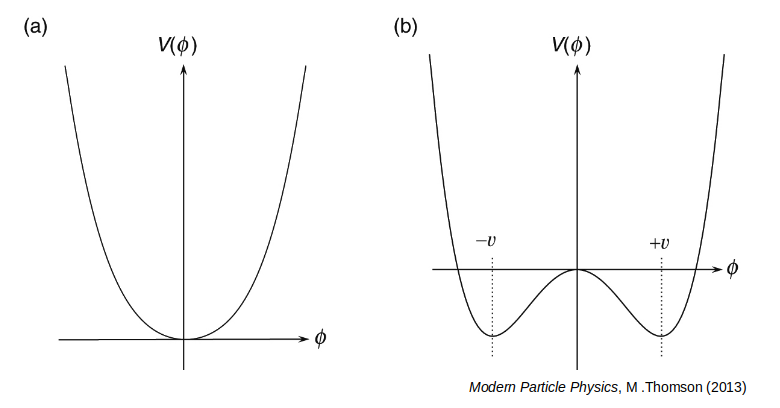
\includegraphics[scale=0.4]{Chapitre2/Images/higgsV1D.png} 
            \caption{Représentation graphique du potentiel $V(\phi)$ pour $\mu^2>0$ (a) et $\mu^2<0$ (b).}
        \label{HiggsV1D}
        \end{figure}

        La valeur non nulle du champ à son minimum de potentiel constitue sa valeur moyenne dans le vide (v.e.v, \textit{vacuum expectation value}), et c'est le choix arbitraire d'une de ses valeurs $\pm\nu$ qui constitue la \textit{brisure de symétrie spontanée} du Lagrangien \ref{laghiggs}. Dans la suite nous considérons une brisure de symétrie vers la valeur positive du champ $+\nu$ et nous introduirons une excitation $\eta(x)$ de ce dernier, assimilée à la création d'une particule, telle que $\phi(x)=\nu+\eta(x)$. Le Lagrangien du champ scalaire devient alors après développement

        \begin{equation*}
        \boxed{
            \mathcal{L}=\frac{1}{2}\bigl(\partial_{\eta}\phi\bigr)\bigl(\partial^{\mu}\eta\bigr)-\lambda\mu^2\eta^2-\lambda\nu\eta^3-\frac{1}{4}\lambda\eta^4+\frac{1}{4}\lambda\nu^4,
        }
        \end{equation*}

        et est constitué des termes suivants :

        \begin{enumerate}
            \item[$\bullet$] $\frac{1}{2}\bigl(\partial_{\eta}\phi\bigr)\bigl(\partial^{\mu}\eta\bigr)$ : terme cinématique associé à $\eta$,
            \item[$\bullet$] $\lambda\mu^2\eta^2$ : terme de masse associé à $\eta$ avec $m_{\eta}=\sqrt{-2\mu^2}$,
            \item[$\bullet$] $\lambda\nu\eta^3,\;\frac{1}{4}\lambda\eta^4$ : interactions à trois et quatre points (fig. \ref{higgsVtx}),
            \item[$\bullet$] $\frac{1}{4}\lambda\nu^4$ : constante sans implication physique.
        \end{enumerate}

        Ce nouveau Lagrangien constitue la représentation physique de l'excitation d'un champ scalaire massif autour de sa valeur moyenne dans le vide après une brisure de symétrie spontanée.

        \begin{figure}
        \centering
            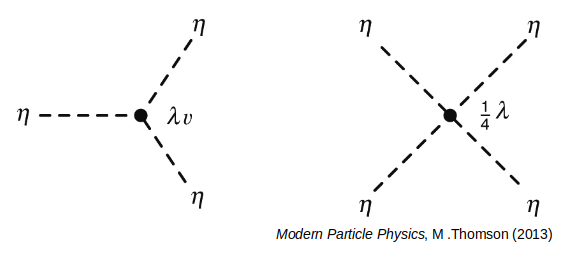
\includegraphics[scale=0.45]{Chapitre2/Images/higgsVtx.png} 
            \caption{Diagrammes de Feynman des auto-interactions du champ scalaire $\eta$ à trois et quatre points.}
        \label{higgsVtx}
        \end{figure}

        \subsection{Mécanisme de Brout-Englert-Higgs (BEH)}
        \label{higgsmeca}

        De façon générale, le mécanisme BEH constitue une démarche visant à introduire une brisure de symétrie spontanée pour un champ scalaire dans une théorie de jauge. Ce processus a pour résultat l'apparition d'un champ de jauge massif dont la nature dépend du groupe de symétrie initialement choisi pour la transformation du Lagrangien, et dont la masse est générée par des interactions avec le champ scalaire. Dans le cas du modèle électrofaible, la théorie de jauge choisie est celle associée au groupe de symétrie SU($2$)$_L\times$U($1$)$_Y$ introduit plus tôt dans le paragraphe \ref{EWK}. Afin d'être compatible avec le nombre de degrés de liberté nécessaire, $\phi$ doit être constitué de deux champs scalaires complexes placés dans un doublet d'isospin faible tel que 

        \begin{equation}
            \phi = \mqty(\phi^+ \\ \phi^0) = \frac{1}{\sqrt{2}}\mqty(\phi_1+i\phi_2 \\ \phi_3 + i\phi_4),
        \label{higgsdoublet}
        \end{equation}

        et dont le Lagrangien s'écrit 

        \begin{equation}
        \begin{array}{ll}
            \mathcal{L}&=\bigl(\partial_{\mu}\phi\bigr)^{\dag}(\partial^{\mu}\phi\bigr)-V(\phi) \vspace{5pt} \\
            &=\bigl(\partial_{\mu}\phi\bigr)^{\dag}(\partial^{\mu}\phi\bigr)-\mu^2\phi^{\dag}\phi-\lambda\bigl(\phi^{\dag}\phi\bigr)^2,
        \end{array}
        \label{HiggsLag}
        \end{equation}

        \begin{figure}
        \centering
            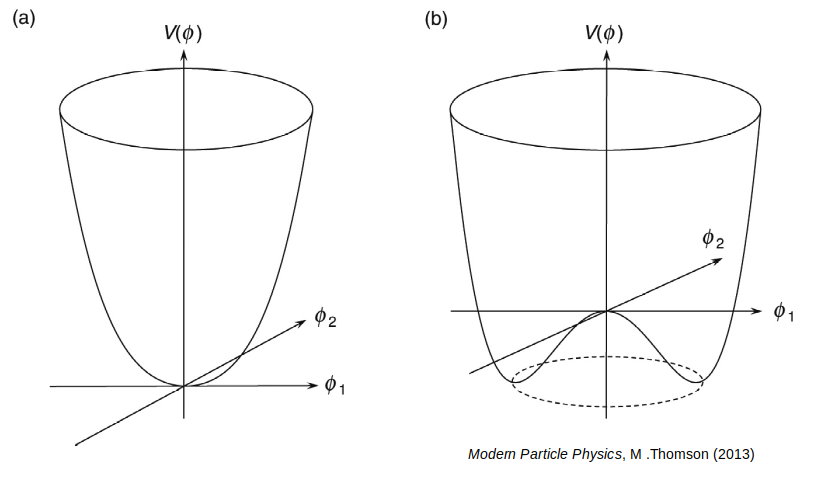
\includegraphics[scale=0.4]{Chapitre2/Images/higgsV3D.png} 
            \caption{Représentation graphique du potentiel de Higgs pour $\mu^2>0$ (a) et $\mu^2<0$ (b).}
        \label{HiggsV3D}
        \end{figure}

        où $V(\phi)$ constitue le potentiel de Higgs avec des paramètres similaires à ceux introduits dans le Lagrangien \ref{laghiggs}. Pour un champ complexe $\phi_1+i\phi_2$, le potentiel présente cette fois une dégénérescence infinie de minima (fig. \ref{HiggsV3D}) pour $\mu^2<0$ sur un cercle satisfaisant l'équation $$\phi_1^2+\phi_2^2=\frac{-\mu^2}{\lambda}=\nu^2.$$ En revanche seul un champ scalaire neutre peut posséder une valeur moyenne dans le vide non nulle afin de conserver la charge électrique et ainsi la v.e.v du doublet d'isospin faible $\phi$ s'écrira $$\ev{\phi}{0}=\frac{1}{\sqrt{2}}\mqty(0 \\ \nu).$$ Après excitation du champ autour de cette dernière, $\phi$ prend alors la forme

        \begin{equation}
            \phi(x)=\frac{1}{\sqrt{2}}\mqty(\phi_1(x)+i\phi_2(x) \\ \nu+\eta(x)+i\phi_4(x)).
        \end{equation}
        
        L'invariance de \ref{HiggsLag} sous une transformation de SU($2$)$_L\times$U($1$)$_Y$ peut quant à elle être conservée en introduisant la dérivée covariante suivante :

        \begin{equation}
            \partial_{\mu}\rightarrow D_{\mu}=\partial_{\mu}+ig_W\vb{T}\cdot\vb{W}_{\mu}+ig'\frac{\mbox{Y}}{2}B_{\mu},
        \label{higgsdcov}
        \end{equation}

        dont les termes sont ceux issus des transformations locales \ref{localSU2} et \ref{localU1Y}. De manière générale, l'ajout d'une dérivée covariante au sein du Lagrangien produit un terme de masse pour les champs de jauge mais également de nouveaux champs reliés à des bosons scalaires sans masse appelés bosons de Goldstone. Ces derniers peuvent se coupler aux champs de jauge grâce à des termes d'interaction à travers lesquels un boson de jauge vectoriel devient scalaire, et n'ont donc pas de réalité physique. Il est toutefois possible de les éliminer avec l'ajout d'une nouvelle jauge, on dit alors que les bosons de Goldstone sont "mangés" par les champs de jauge. Ce mécanisme entraîne l'apparition d'un nouveau degré de polarisation longitudinal des bosons de jauge correspondant au troisième degré de projection du spin $S_z=0$ propre aux particules massives de spin $1$. En réalité la démarche visant à éliminer les bosons de Goldstone peut être contournée en évitant leur apparition avec le même résultat final en choisissant initialement une jauge dite unitaire pour le champ scalaire telle que seul le champ d'excitation persiste et soit purement réel. Dans le cas du mécanisme BEH électrofaible on obtient alors :

        \begin{equation}
            \phi=\frac{1}{\sqrt{2}}\mqty(0 \\ \nu+h(x)),
        \label{higgsunit}
        \end{equation}

        où $h(x)$ désigne cette fois le \textit{champ de Higgs}. La masse des bosons de jauge peut être déterminée à partir du terme cinétique du Lagrangien $\bigl(D_{\mu}\phi\bigr)^{\dag}\bigl(D^{\mu}\phi\bigr)$ dans lequel ont été introduits la dérivée covariante \ref{higgsdcov} et la jauge unitaire \ref{higgsunit} :

        \begin{equation*}
        \begin{array}{ll}
            \bigl(D_{\mu}\phi\bigr)^{\dag}\bigl(D^{\mu}\phi\bigr) = & \frac{1}{2}\bigl(\partial_{\mu}h\bigr)\bigl(\partial^{\mu}h\bigr) \vspace{5pt} \\
            & +\frac{1}{8}g_W^2\bigl(W^{(1)}_{\mu}+iW^{(2)}_{\mu}\bigr)\bigl(W^{(1),\mu}-iW^{(2),\mu}\bigr)(\nu+h)^2 \vspace{5pt} \\
            & +\frac{1}{8}\bigl(g_WW^{(3)}_{\mu}-g'B_{\mu}\bigr)\bigl(g_WW^{(3),\mu}-g'B^{\mu}\bigr)(\nu+h)^2.
        \end{array}
        \end{equation*}

        On reconnaît en particulier dans le second terme de ce résultat la double combinaison des champs $W^{(1)}$ et $W^{(2)}$ dont la structure est semblable à celle des courants chargés \ref{Wexchange} associés à l'échange des bosons $W^{\pm}$. Afin de déterminer les termes de masse, il convient de développer les termes quadratiques dans lesquels interviennent les champs de jauge. De cette façon nous obtenons pour les bosons $W^{\pm}$ :

        \begin{equation*}
        \begin{array}{ll}
            \frac{1}{8}\nu^2g^2_W\bigl(W^{(1)}_{\mu}W^{(1),\mu}&+W^{(2)}_{\mu}W^{(2),\mu}\bigr) \vspace{5pt}\\
            &=\frac{1}{2}m^2_W\bigl(W^{(1)}_{\mu}W^{(1),\mu}+W^{(2)}_{\mu}W^{(2),\mu}\bigr),
        \end{array}
        \end{equation*}

        avec

        \begin{equation}
            \boxed{
            m_W=\frac{1}{2}g_W\nu.
            }
        \end{equation}

        Le terme associé aux champs $W_{\mu}^{(3)}$ et $B_{\mu}$ peut quant à lui s'écrire sous la forme matricielle suivante :

        \begin{equation*}
        \begin{array}{ll}
            \frac{\nu^2}{8}\mqty(W^{(3)}_{\mu}&&B_{\mu})&\mqty(g^2_W&&-g_Wg'\\-g_Wg'&&g'^2)\mqty(W^{(3),\mu}\\B^{\mu}) \vspace{5pt} \\
            &=\frac{\nu^2}{8}\mqty(W^{(3)}_{\mu}&&B_{\mu})\vb{M}\mqty(W^{(3),\mu}\\B^{\mu}),
        \end{array}
        \end{equation*}

        où $\vb{M}$ représente une matrice non-diagonale de masse à travers laquelle les champs $W_{\mu}^{(3)}$ et $B_{\mu}$ se mélangent. En opérant un changement de base dans laquelle cette matrice est diagonale, il est alors possible de définir la structure des champs correspondant à des bosons physiques dont les masses seront données par les termes diagonaux $\lambda$ de $\vb{M}$ obéissant à l'équation $\det(\vb{M}-\lambda I)=0$. Dans le cas de l'interaction électrofaible, les bosons physiques recherchés correspondent au photon et au boson $Z^0$, respectivement associés aux champs $A_{\mu}$ et $Z_{\mu}$ introduits plus tôt. Dans la nouvelle base on obtient alors :

        \begin{equation*}
        \begin{array}{ll}
            \frac{\nu^2}{8}\mqty(A_{\mu}&&Z_{\mu})&\mqty(0&&0\\0&&g^2_W+g'^2)\mqty(A^{\mu}\\Z^{\mu}) \vspace{5pt} \\
            &=\frac{1}{2}\mqty(A_{\mu}&&Z_{\mu})\mqty(m_A^2&&0\\0&&m_Z^2)\mqty(A^{\mu}\\Z^{\mu}),
        \end{array}
        \end{equation*}    

        et ainsi 

        \begin{equation}
            \boxed{
            m_A=0 \quad \mbox{et} \quad m_Z=\frac{1}{2}\nu\sqrt{g^2_W+g'^2}.
            }
        \end{equation}

        Il est alors intéressant de noter que tandis que le photon reste sans masse après brisure de symétrie, les bosons de l'interaction faible ont acquis une masse dont la valeur est proportionnelle à la valeur moyenne dans le vide du champ de Higgs. Le Lagrangien contient également désormais des termes d'interaction dont la structure permet de définir les diagrammes de Feynman présents dans la figure \ref{higgsVcoupling}

        \begin{figure}
        \centering
            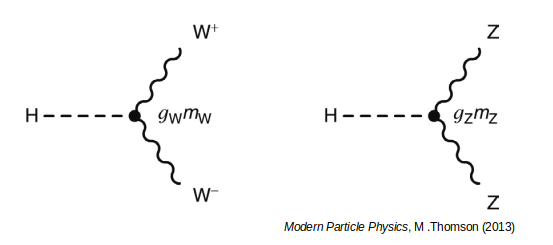
\includegraphics[scale=0.45]{Chapitre2/Images/higgsVcoupling.png} 
            \caption{Diagrammes de Feynman des couplages entre le boson de Higgs $H$ et les bosons $W^{\pm}$ et $Z^0$.}
        \label{higgsVcoupling}
        \end{figure}
        
        \subsection{Couplages de Yukawa}
        \label{yukawa}

        \begin{figure}
        \centering
            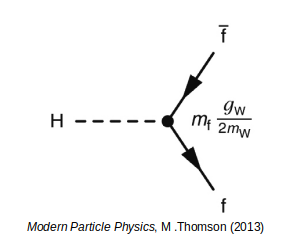
\includegraphics[scale=0.45]{Chapitre2/Images/higgsfcoupling.png} 
            \caption{Diagramme de Feynman du couplage entre le boson de Higgs $H$ et les fermions.}
        \label{higgsfcoupling}
        \end{figure}

        Le mécanisme de Higgs introduit dans la partie précédente permet de déterminer l'origine de la masse des bosons de l'interaction faible et de leur degré supplémentaire de polarisation longitudinale tout en conservant l'absence de masse du photon. En revanche l'origine de la masse des fermions reste inexpliquée à ce stade. Le terme de masse associé aux fermions dans le Lagrangien de Dirac peut être exprimé en fonction des composantes chirales gauche et droite des spineurs de Dirac $\psi$ de façon à obtenir $$-m\overline{\psi}\psi=m\bigl(\overline{\psi}_R\psi_L+\overline{\psi}_L\psi_R\bigr).$$ Ce terme n'est cependant pas invariant sous une transformation du groupe de symétrie SU($2$)$_L\times$U($1$)$_Y$. De la même façon que lors de l'introduction de l'unification électrofaible dans la partie \ref{EWK}, les fermions de chiralité gauche $\psi_L$ sont placés dans des doublets de SU($2$), tandis que les fermions de chiralité droite $\psi_R$ sont placés dans des singlets. Puisque les champs complexes \ref{higgsdoublet} du mécanisme BEH sont eux aussi placés dans un doublet $\phi$, la combinaison $\overline{\psi}_L\phi$ de ce dernier avec $\psi_L$ est elle aussi invariante sous une transformation de SU($2$). Il est alors possible de définir une forme de couplage invariante sous une transformation de SU($2$)$_L\times$U($1$)$_Y$ à partir d'une combinaison du terme précédent avec un singlet $\psi_R$ et une constante de couplage propre à chaque fermion s'écrivant $-g_f\bigl(\overline{\psi}_L\phi\psi_R+\overline{\psi}_R\phi^{\dag}\psi_L\bigr)$. En choisissant un exemple à partir du doublet et du singlet contenant l'électron et en appliquant à $\phi$ la jauge unitaire \ref{higgsunit}, le Lagrangien associé peut s'écrire sous la forme

        \begin{align*}
             \mathcal{L}_e & = -\frac{g_e}{\sqrt{2}}\mqty[\mqty(\overline{\nu}_e&&\overline{e})_L\mqty(0\\\nu+h(x))e_R+\overline{e}_R\mqty(0&&\nu+h(x))\mqty(\nu_e\\e)_L] \vspace{5pt} \\
             & = -\frac{g_e}{\sqrt{2}}\nu\bigl(\overline{e}_Le_R+\overline{e}_Re_L\bigr)-\frac{g_e}{\sqrt{2}}h\bigl(\overline{e}_Le_R+\overline{e}_Re_L\bigr) \vspace{5pt} \\
             & = -\frac{g_e}{\sqrt{2}}\bigl(\nu\overline{e}e+h\overline{e}e\bigr).
        \end{align*}

        La valeur de la constante de couplage présente dans le Lagrangien n'étant pas prédite par le mécanisme BEH, elle est librement choisie comme étant reliée à la masse $m_e$ de l'électron et telle que $$g_e=\sqrt{2}\frac{m_e}{\nu}.$$ Le Lagrangien peut alors être étendu à tous les fermions avec la forme générale

        \begin{equation}
        \boxed{
            \mathcal{L}_f=-\frac{g_f}{\sqrt{2}}\bigl(\nu\overline{\psi}\psi+h\overline{\psi}\psi\bigr) \vspace{5pt}=-m_f\overline{\psi}\psi-\frac{m_f}{\nu}\overline{\psi}\psi h
        ,}
        \label{yukawacoupling}
        \end{equation}

        où $g_f$ représente les \textit{couplages de Yukawa} des fermions. Le second terme illustre le couplage entre le boson de Higgs et les fermions dont le diagramme de Feynman est donné dans la figure \ref{higgsfcoupling}.



        
